\documentclass[conference]{IEEEtran}
\IEEEoverridecommandlockouts

\usepackage{cite}
\usepackage{amsmath,amssymb,amsfonts}
\usepackage{algorithmic}
\usepackage{graphicx}
\usepackage{textcomp}
\usepackage{xcolor}
\usepackage{booktabs}
\usepackage{multirow}
\usepackage{url}

\def\BibTeX{{\rm B\kern-.05em{\sc i\kern-.025em b}\kern-.08em
    T\kern-.1667em\lower.7ex\hbox{E}\kern-.125emX}}

\begin{document}

\title{Cycle-Time Optimization of Reconfigurable Robotic Pick-and-Place Cells in a Digital Twin}

% Authors intentionally omitted for now.
\author{}

\maketitle

\begin{abstract}
Layout design for robotic pick-and-place cells is dominated by the cost of evaluating
candidate configurations: each evaluation conventionally requires a sampling-based motion
plan in a high-fidelity simulator, which is both slow and stochastic. We present a
declarative reconfigurable-cell framework (ROS\,2 Jazzy + Gazebo Harmonic + MoveIt\,2,
UR5 + RG2 gripper) in which an optimizer searches over station poses and visit order using
a \emph{deterministic joint-travel surrogate} as its objective, rather than the simulator.
The surrogate evaluates a configuration by chaining canonical, elbow-up inverse-kinematics
solutions and summing joint-space travel, achieving $<\!0.0003\%$ run-to-run spread. Our
central contribution is an \emph{honest} validation of this surrogate against real planned
motion time. A naive comparison against a randomized feasibility planner (RRTConnect) yields
no reliable correlation---the Pearson coefficient flips sign between repetitions
($+0.057$ vs.\ $-0.550$)---because per-plan path-length variance ($\sim\!96\%$) swamps the
between-configuration signal. Once the measurement is aligned with what the surrogate models
---an \emph{optimizing} planner (RRTstar), kinematic \emph{continuity} (joint-to-joint
goals), and a fixed visit order---the surrogate strongly predicts converged-optimal motion
time: Pearson $r=0.880$, Spearman $\rho=0.943$ ($n=6$). Optimizing against the surrogate with
simulated annealing beats an equal-budget random baseline $5/5$ (mean $-17.4\%$), and the
predicted reduction transfers to real motion: pooled $r=0.876$, with optimized configurations
running $19.4\%$ faster in real RRTstar motion. Finally, an optimized configuration executes a
full pick--place--pick--place relay end-to-end in the high-fidelity twin (two clean trials,
no planning failures). We also report the boundary of the result: the most aggressive
minimal-travel layouts are infeasible for the twin's default randomized planner, so
time \emph{prediction} and full-twin \emph{executability} are distinct guarantees.
\end{abstract}

\begin{IEEEkeywords}
robotic cell design, motion planning, digital twin, simulated annealing, surrogate
optimization, reconfigurable manufacturing.
\end{IEEEkeywords}

\section{Introduction}
The throughput of a robotic pick-and-place cell is largely fixed at design time by the
relative placement of its work stations and the order in which the robot visits them.
Searching this layout space is attractive but expensive: the natural objective---real cycle
time---is obtained only by executing or planning each candidate in a simulator. Sampling-based
planners such as RRTConnect~\cite{rrtconnect} are fast but stochastic, so a single
configuration must be evaluated many times to average out path-length variance, and a global
search over hundreds of candidates becomes intractable.

A common remedy is a cheap surrogate objective. The risk is that the surrogate optimizes a
proxy that does not track the quantity of interest. This paper takes the validation of that
proxy as seriously as the optimization itself. We build a declarative, reconfigurable cell on
ROS\,2 and Gazebo (Section~\ref{sec:system}), define a deterministic joint-travel surrogate
(Section~\ref{sec:surrogate}), and then ask---repeatedly and honestly---whether it predicts
real planned motion time (Section~\ref{sec:gate}). We deliberately report two failed attempts
before the successful one, because the failure mode is instructive: the surrogate is only
predictive when the measurement is methodologically aligned with what it models. We then
optimize against the validated surrogate and confirm that the predicted gains transfer both to
real planned motion (Section~\ref{sec:loop}) and to full execution in the high-fidelity twin
(Section~\ref{sec:twin}).

\textbf{Contributions.} (i)~A declarative reconfigurable-cell framework with a reusable
headless IK oracle shared between synthesis and simulation. (ii)~A deterministic joint-travel
surrogate with $<\!0.0003\%$ spread, suitable as a stable optimization objective.
(iii)~A rigorous surrogate-to-real validation establishing that the surrogate predicts an
\emph{optimizing} planner's motion time ($r=0.88$), together with a clear account of why it
fails against a randomized planner. (iv)~An end-to-end demonstration that simulated-annealing
optimization against the surrogate yields configurations that are faster in real motion and
executable in the twin, and an honest characterization of where executability breaks down.

\section{System Architecture}
\label{sec:system}
The platform is a digital twin built on ROS\,2 Jazzy and Gazebo Harmonic, with a Universal
Robots UR5 arm and an OnRobot RG2 two-finger gripper (Fig.~\ref{fig:overview}). Motion planning
uses MoveIt\,2 with the OMPL planner suite. A cell is described declaratively in a locked
schema---robot mount pose, belt geometry, part geometry, and a list of conveyor \emph{stations}
(each with an $(x,y,\psi)$ pose), plus a relay \emph{task} as an ordered list of pick/place
operations. A generator realizes a configuration document into a \texttt{scene.yaml} and
\texttt{task.yaml} consumed by the simulation.

\begin{figure}[t]
\centering
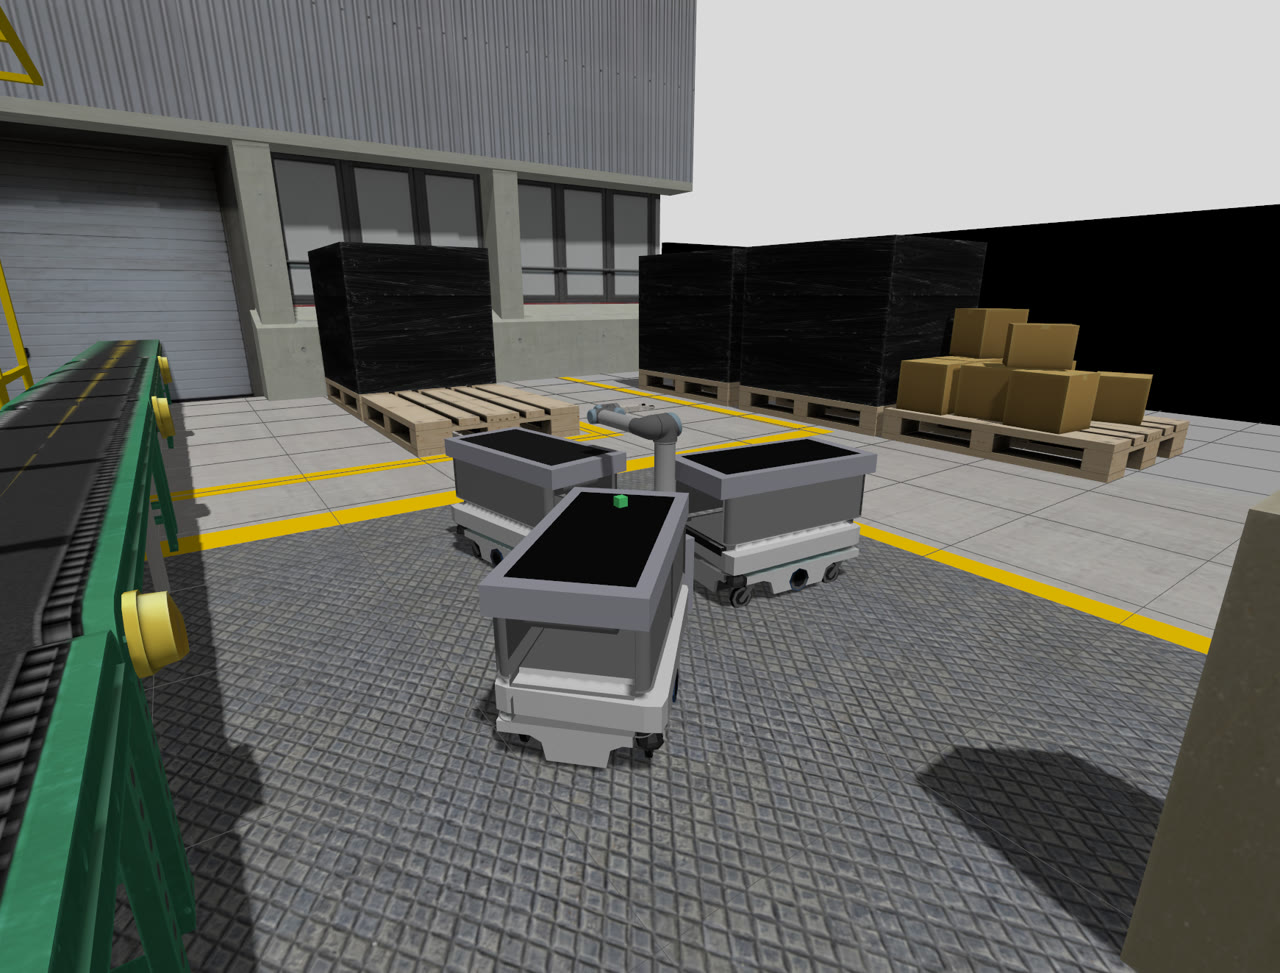
\includegraphics[width=\columnwidth]{figs/twin_overview.jpg}
\caption{The high-fidelity Gazebo Harmonic twin for an optimized configuration
(\texttt{val\_0}): a UR5\,+\,RG2 arm on a pedestal serves three conveyor stations against a
warehouse backdrop. Station poses and visit order are produced by the optimizer; the green cube
is the transferred part.}
\label{fig:overview}
\end{figure}

Two components are shared, by import, between the headless optimizer and the live simulator,
which is what makes the surrogate trustworthy: (1)~an \emph{IK reachability guard} that rejects
any configuration with an unreachable station, and (2)~the inverse-kinematics oracle used to
score configurations. Grasping in the twin is implemented as a welded detachable joint, so the
focus of this study is reach and transit motion rather than contact dynamics.

A practical but important lesson during twin construction: the \texttt{ros\_gz\_sim} spawn
utility silently ignores a pose embedded in an SDF string, so every runtime fixture must be
spawned via explicit \texttt{-x/-y/-z/-Y} flags; otherwise all fixtures stack at the world
origin. Belt-support slabs are added so the part rests at a stable grasp height.

\section{Deterministic Joint-Travel Surrogate}
\label{sec:surrogate}
The surrogate estimates the motion cost of a configuration without invoking a planner. For each
target pose in the (ordered) relay, it computes inverse kinematics and selects the
\emph{canonical} solution---the collision-free branch closest to a fixed elbow-up seed over a
deterministic seed bank---then sums the joint-space distance traveled between consecutive
canonical configurations. Selecting a canonical branch is essential: a generic IK call random-
restarts and jumps between elbow-up/elbow-down solutions, which made an early version of the
surrogate vary by $50$--$127\%$ on identical inputs. With canonical selection the surrogate is
effectively deterministic, with measured run-to-run spread below $0.0003\%$. This stability is a
prerequisite for using it as an optimization objective: simulated annealing requires that two
evaluations of the same point return the same value.

The visit order is fixed separately by a brute-force traveling-salesman solution over the
stations, so that the surrogate and any downstream real measurement use an identical order.

\section{Surrogate-to-Real Validation}
\label{sec:gate}
We treat ``does the surrogate predict real motion time?'' as a hard gate that must pass before
any optimization result is trusted. The validation set \texttt{val\_hb} contains six valid
configurations spanning a range of surrogate values, all sharing one robot mount.

\subsection{Two honest negatives}
\textbf{Attempt 1 (inconclusive).} Measuring full cycle time in the twin mixed in
$\sim\!130$\,s of configuration-independent reset/settle overhead and suffered $\sim\!2\times$
run-to-run motion variance from the randomized planner; no clean trend emerged, and sim
instability prevented collecting enough runs to average it out.

\textbf{Attempt 2 (reliable negative).} A headless probe stripped the fixed overhead and the
wall-clock noise by summing planned trajectory \emph{duration} with the real RRTConnect planner,
averaged best-of-10. The result was explicitly \emph{not} a relationship: the Pearson coefficient
flipped sign between repetitions of the same experiment ($+0.057$ at 12 plans vs.\ $-0.550$ at 40
plans). The cause is that RRTConnect path duration retains $\sim\!96\%$ per-plan spread even at
best-of-10, and frequently fails on the collision-constrained reaches. A coefficient that flips
sign is measuring noise; we report it as such rather than selecting the favorable run.

\subsection{Aligning the measurement (Attempt 3)}
The diagnosis was that minimal joint travel is the wrong target for a \emph{randomized,
feasibility-only} sampler. Three changes align the real measurement with the quantity the
surrogate models:
\begin{enumerate}
\item \textbf{Optimizing planner.} RRTConnect $\rightarrow$ RRTstar~\cite{rrtstar}, which is
asymptotically optimal in path cost. This required injecting a group-qualified planner
configuration so RRTstar is selectable for the arm group.
\item \textbf{Kinematic continuity.} The relay is planned joint-to-joint: each station's goal is
the collision-free IK branch closest to the previous station's joint state, eliminating spurious
elbow-flip excursions. A transfer $A\rightarrow B$ excludes \emph{both} endpoint belts (leaving
$A$ and approaching $B$ are required, not collisions), while every other belt remains an obstacle.
\item \textbf{Fixed visit order.} The brute-force TSP order is shared by surrogate and real
measurement.
\end{enumerate}
With continuity, five of six configurations become near-deterministic (per-plan spread
$89\%\rightarrow0\%$); the lone exception, \texttt{val\_2}, is RRTstar occasionally failing to
converge to its optimum.

\subsection{Result}
Table~\ref{tab:gate} reports the surrogate and the real RRTstar motion time (minimum, mean,
median, std over 10 plans). Because RRTstar is asymptotically optimal, the \emph{minimum}
planned duration is the best estimate of its converged-optimal path cost; the mean is
contaminated by non-converged runs (visibly \texttt{val\_2}, whose min $7.35$\,s matches its
mid-range surrogate while unlucky runs inflate its mean to $12.6$\,s). Table~\ref{tab:estimators}
compares correlation under each estimator; the min is both the most principled and the strongest.
Fig.~\ref{fig:gate} shows the scatter and fit.

\begin{table}[t]
\caption{Surrogate vs.\ real RRTstar motion time on \texttt{val\_hb} ($n=6$,
RRTstar $6$\,s $\times\,10$ plans). Min is the converged-optimal estimate.}
\label{tab:gate}
\centering
\begin{tabular}{lccccc}
\toprule
config & surrogate & min (s) & mean (s) & median (s) & std \\
\midrule
val\_0 & 5.17 & \textbf{6.81} & 6.81 & 6.81 & 0.00 \\
val\_1 & 6.38 & \textbf{8.06} & 9.14 & 8.92 & 0.98 \\
val\_2 & 6.60 & \textbf{7.35} & 12.58 & 10.40 & 3.79 \\
val\_4 & 6.92 & \textbf{8.56} & 8.61 & 8.61 & 0.02 \\
val\_3 & 6.96 & \textbf{9.03} & 9.08 & 9.10 & 0.03 \\
val\_5 & 7.36 & \textbf{9.11} & 9.52 & 9.11 & 1.22 \\
\bottomrule
\end{tabular}
\end{table}

\begin{table}[t]
\caption{Correlation of the surrogate with real motion time, by estimator.}
\label{tab:estimators}
\centering
\begin{tabular}{lcc}
\toprule
estimator & Pearson $r$ & Spearman $\rho$ \\
\midrule
\textbf{min} (converged-optimal) & \textbf{0.880} & \textbf{0.943} \\
median & 0.704 & 0.543 \\
mean & 0.486 & 0.371 \\
\bottomrule
\end{tabular}
\end{table}

\begin{figure}[t]
\centering
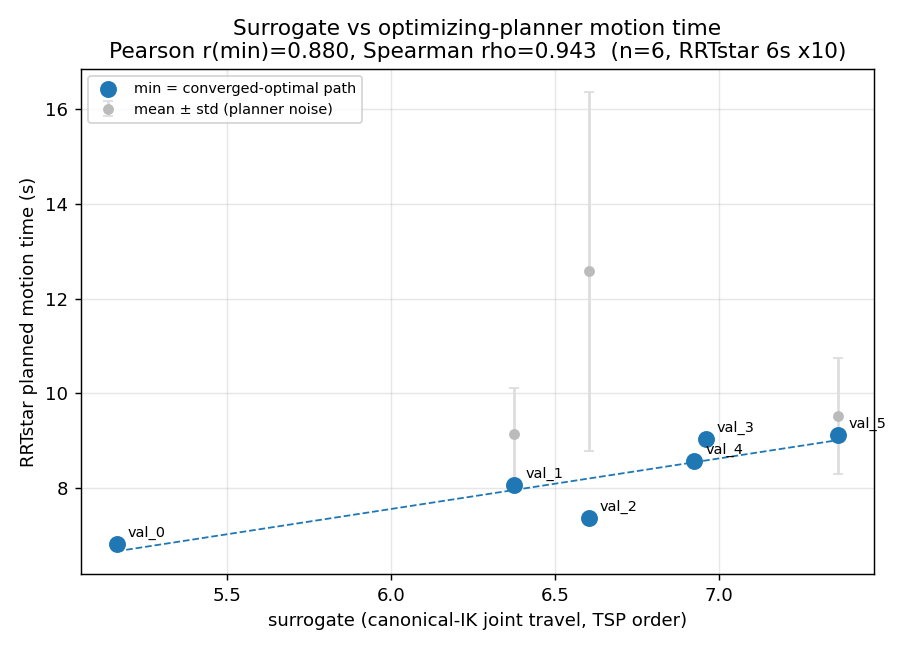
\includegraphics[width=0.92\columnwidth]{figs/gate_scatter.png}
\caption{Surrogate vs.\ real RRTstar motion time on \texttt{val\_hb}. Filled points and fit line
use the converged-optimal (min) estimate ($r=0.880$, $\rho=0.943$); faded points show
mean\,$\pm$\,std for transparency.}
\label{fig:gate}
\end{figure}

Once the measurement matches what the surrogate models, the deterministic joint-travel surrogate
strongly predicts the optimizing planner's motion time, and the rank order is almost exact
($\rho=0.943$). Attempt~2's negative is therefore a property of the randomized planner/sampler,
not of the surrogate. The gate passes, justifying optimization against the surrogate.

\section{Cycle-Time Optimization and Closing the Loop}
\label{sec:loop}
\subsection{Simulated annealing against the surrogate}
We optimize station poses $(x,y,\psi)$ and visit order with simulated
annealing~\cite{simanneal}. Moves comprise order swaps, global jumps, and local nudges, annealed
with a cooling temperature and reheating; the search is seeded from the best of several random
valid configurations. The fair baseline is the best random-valid configuration found under an
\emph{identical} oracle-evaluation budget, so any improvement is attributable to the search, not
to extra evaluations. Across five specifications (5 seeds, 400 iterations, three stations),
simulated annealing beats the equal-budget random baseline $5/5$, with a mean improvement of
$17.4\%$ (Table~\ref{tab:sa}, Fig.~\ref{fig:sa}).

\begin{table}[t]
\caption{Simulated annealing vs.\ equal-budget random baseline (3 stations, 400 iters).}
\label{tab:sa}
\centering
\begin{tabular}{lcccc}
\toprule
seed & SA cost & baseline & impr.\ vs.\ base & best order \\
\midrule
100 & 4.750 & 6.491 & $26.8\%$ & c3\,$|$\,c1\,$|$\,c2 \\
101 & 4.453 & 6.154 & $27.7\%$ & c3\,$|$\,c1\,$|$\,c2 \\
102 & 4.468 & 5.210 & $14.2\%$ & c2\,$|$\,c1\,$|$\,c3 \\
103 & 4.774 & 5.355 & $10.8\%$ & c1\,$|$\,c3\,$|$\,c2 \\
104 & 4.887 & 5.287 & $7.6\%$ & c1\,$|$\,c3\,$|$\,c2 \\
\midrule
mean & 4.667 & 5.699 & \textbf{$17.4\%$} & --- \\
\bottomrule
\end{tabular}
\end{table}

\begin{figure*}[t]
\centering
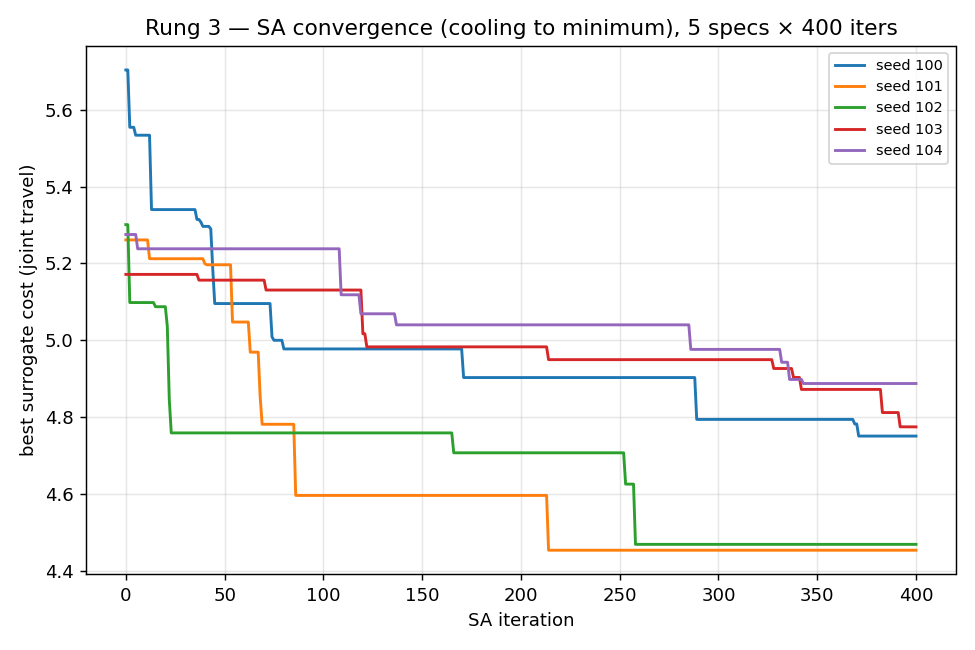
\includegraphics[width=0.46\textwidth]{figs/sa_convergence.png}\hfill
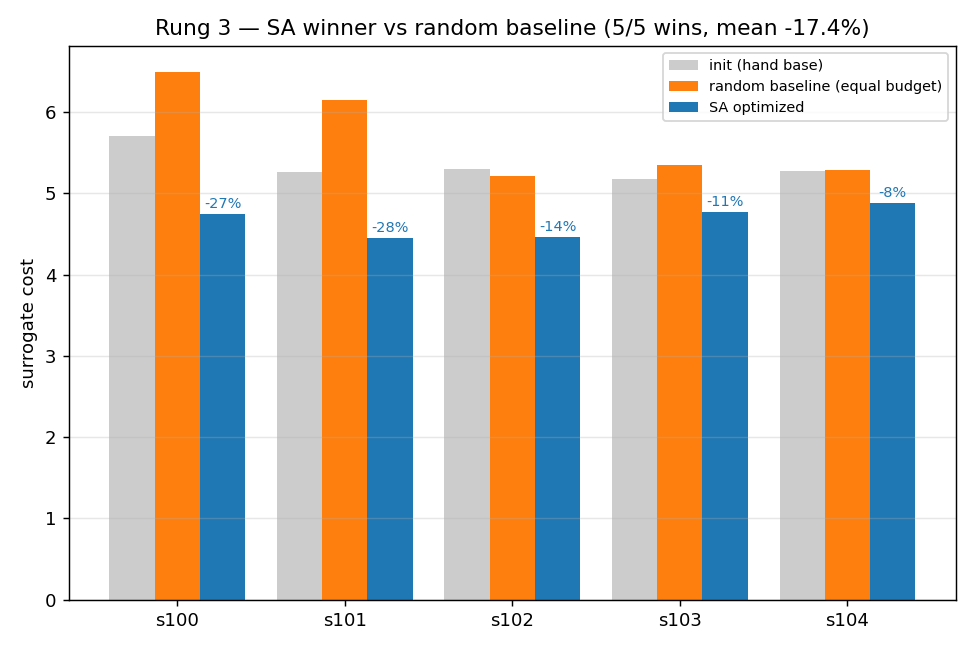
\includegraphics[width=0.46\textwidth]{figs/sa_vs_baseline.png}
\caption{Simulated annealing against the surrogate. Left: convergence trajectories (surrogate
cost vs.\ iteration) for the five seeds, cooling to a global minimum. Right: final optimized cost
vs.\ the equal-budget random baseline per seed; SA wins $5/5$ (mean $-17.4\%$).}
\label{fig:sa}
\end{figure*}

\subsection{The predicted reduction transfers to real motion}
We then run the five optimized winners back through the headless RRTstar probe and pool them with
the six prior valid configurations ($n=11$). The correlation holds on min motion (Pearson
$r=0.876$, Spearman $\rho=0.900$). All five optimized winners are perfectly deterministic over 10
plans (std $0.00$) and sit at the low real-motion end. Their mean real motion is $6.79$\,s versus
$8.42$\,s for the random valids---a $19.4\%$ reduction that empirically matches the $-17.4\%$
surrogate gain (Table~\ref{tab:loop}, Fig.~\ref{fig:loop}). The loop is closed: a reduction in the
cheap surrogate produces a reduction in real optimizing-planner motion of the same magnitude.

\begin{table}[t]
\caption{Closed loop: optimized winners vs.\ random valids (pooled $n=11$, min motion).}
\label{tab:loop}
\centering
\begin{tabular}{lcc}
\toprule
group & mean real motion (s) & pooled correlation \\
\midrule
SA winners ($n=5$) & \textbf{6.79} & \multirow{2}{*}{$r=0.876,\ \rho=0.900$} \\
random valids ($n=5$) & 8.42 & \\
\midrule
\multicolumn{3}{c}{relative improvement: \textbf{$-19.4\%$} real motion ($-17.4\%$ surrogate)} \\
\bottomrule
\end{tabular}
\end{table}

\begin{figure}[t]
\centering
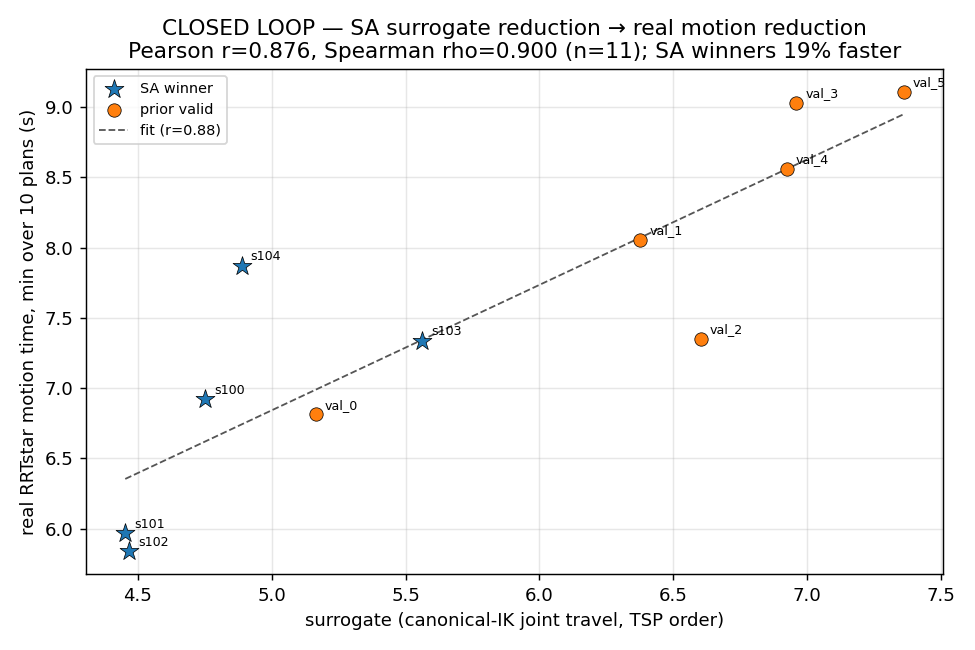
\includegraphics[width=0.92\columnwidth]{figs/closed_loop.png}
\caption{Pooled surrogate vs.\ real motion ($n=11$). Optimized winners (low end) and random
valids lie on the same trend; the surrogate reduction maps onto a real-motion reduction.}
\label{fig:loop}
\end{figure}

\section{High-Fidelity Twin Execution}
\label{sec:twin}
To confirm that an optimized configuration is not merely fast on paper, we executed a feasible
optimized winner (\texttt{val\_0}, surrogate $5.19$) in the full high-fidelity twin: Gazebo
Harmonic GUI, the complete \texttt{move\_group} stack, the real RG2 gripper, and a welded-cube
carry. The IK guard passed (all three stations reachable), and the four-operation relay
(pick--place--pick--place) ran end-to-end across a warmup and a measured trial, both succeeding
with the gripper verified clear at start and no planning failures
(Table~\ref{tab:twin}, Fig.~\ref{fig:relay}).

\begin{figure}[t]
\centering
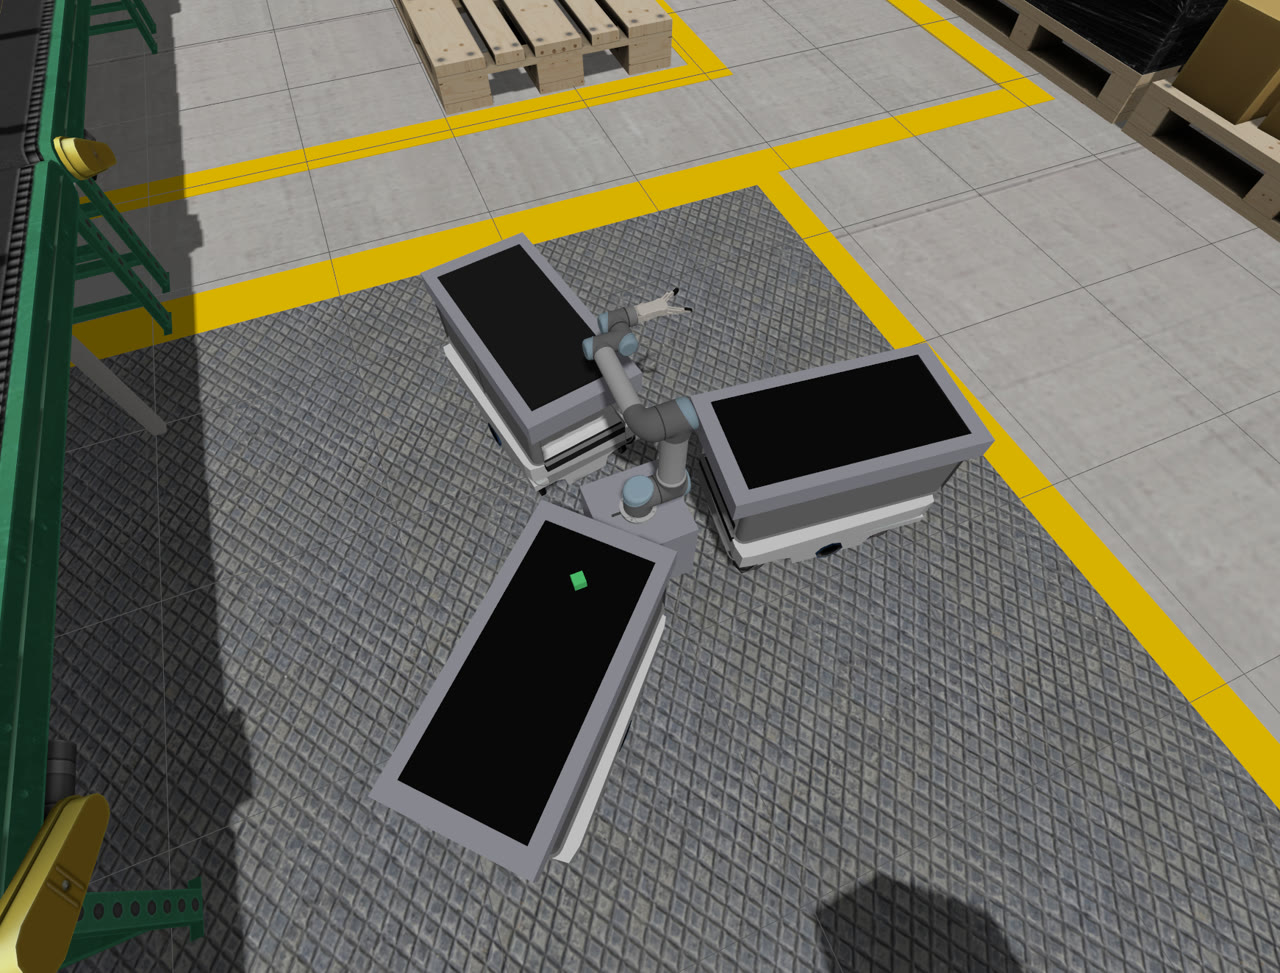
\includegraphics[width=\columnwidth]{figs/twin_relay.jpg}
\caption{Twin execution of the optimized winner \texttt{val\_0}: the UR5\,+\,RG2 arm reaches into
a conveyor station mid-relay. The three stations are pinwheeled around the arm in the optimizer's
chosen layout; the welded part (green cube) is carried between stations. Both trials complete the
full pick--place--pick--place relay with no planning failures (Table~\ref{tab:twin}).}
\label{fig:relay}
\end{figure}

\begin{table}[t]
\caption{Full-twin relay execution of optimized winner \texttt{val\_0}.}
\label{tab:twin}
\centering
\begin{tabular}{lcccc}
\toprule
run & cycle (s) & success & gripper clear & failure \\
\midrule
warmup & 133.0 & yes & yes & none \\
trial 1 & 148.0 & yes & yes & none \\
\bottomrule
\end{tabular}
\end{table}

\section{Discussion and Limitations}
The result is bounded in an important way. The most \emph{aggressive} minimal-travel winners
produced by the optimizer place stations close together; while the headless RRTstar probe (with
belt exclusion and joint continuity) solves these, the twin's default randomized planner
(RRTConnect with the real gripper collision model and a welded carry) cannot execute the cramped
later segments---the first transfer succeeds, then a subsequent segment fails to plan. Thus our
guarantees separate cleanly: the surrogate is validated as a predictor of optimizing-planner
\emph{motion time}, and an optimized configuration is demonstrated \emph{executable} in the twin,
but the single most aggressive optimum is not necessarily both. A natural extension is to fold a
twin-executability constraint (e.g., a minimum inter-station clearance, or planning with the same
planner the twin uses) directly into the surrogate or as an optimization constraint. Other
limitations include welded grasping (contact dynamics are out of scope) and a three-station relay;
scaling the station count and the part set is future work.

\section{Conclusion}
We presented a reconfigurable robotic pick-and-place cell whose layout is optimized against a
deterministic joint-travel surrogate, and validated that surrogate against a high-fidelity twin
with explicit attention to honesty: two documented negative results precede the positive one, and
the boundary of the positive result is stated. When the real measurement is aligned with what the
surrogate models---an optimizing planner, kinematic continuity, and a fixed visit order---the
surrogate predicts converged-optimal motion time ($r=0.88$, $\rho=0.94$). Simulated annealing
against the surrogate beats an equal-budget baseline $5/5$ ($-17.4\%$), and the gain transfers to
real motion ($-19.4\%$) and to a clean end-to-end relay in the twin. The methodology---validate
the proxy as rigorously as the optimization, and report where it stops holding---is the central
takeaway.

\begin{thebibliography}{1}
\bibitem{rrtconnect}
J.~J. Kuffner and S.~M. LaValle, ``RRT-Connect: An efficient approach to single-query path
planning,'' in \emph{Proc. IEEE Int. Conf. Robot. Autom. (ICRA)}, 2000, pp.~995--1001.

\bibitem{rrtstar}
S.~Karaman and E.~Frazzoli, ``Sampling-based algorithms for optimal motion planning,''
\emph{Int. J. Robot. Res.}, vol.~30, no.~7, pp.~846--894, 2011.

\bibitem{simanneal}
S.~Kirkpatrick, C.~D. Gelatt, and M.~P. Vecchi, ``Optimization by simulated annealing,''
\emph{Science}, vol.~220, no.~4598, pp.~671--680, 1983.

\bibitem{moveit}
D.~Coleman, I.~Sucan, S.~Chitta, and N.~Correll, ``Reducing the barrier to entry of complex
robotic software: a MoveIt! case study,'' \emph{J. Softw. Eng. Robot.}, vol.~5, no.~1,
pp.~3--16, 2014.

\bibitem{ompl}
I.~A. \c{S}ucan, M.~Moll, and L.~E. Kavraki, ``The Open Motion Planning Library,''
\emph{IEEE Robot. Autom. Mag.}, vol.~19, no.~4, pp.~72--82, 2012.

\bibitem{ros2}
S.~Macenski, T.~Foote, B.~Gerkey, C.~Lalancette, and W.~Woodall, ``Robot Operating System~2:
Design, architecture, and uses in the wild,'' \emph{Sci. Robot.}, vol.~7, no.~66, 2022.
\end{thebibliography}

\end{document}
